%Encoding: utf-8
%Projekt 5. do predmetu ITY
%Autor: Pavol Loffay, 1. rocnik BIB-30, xloffa00@stud.fit.vutbr.cz
%Datum: 21.4.2011

\documentclass[pdf,fyma2, total]{prosper}

%\usepackage[IL2]{fontenc} %TODO NEEFUNGUJE
\usepackage[utf8]{inputenc}
\usepackage[slovak]{babel}

\usepackage{graphics}
%vektorovy obrazok
\usepackage{picture}

%ako sa maju slidi zobrazovat
\DefaultTransition{Split}

%cislovanie stran v patke dokumentu
\slideCaption{Typografia a publikovanie 5. projekt Športové Lezenie}

%textova cast
\begin{document}

\begin{titlepage}
	\title{Typografia a publikovnie 5. projekt}
	\subtitle{Športové lezenie}
	\author{Pavol Loffay}
	\email{xloffa00@stud.fit.vutbr.cz}
	\date{\today}
	\maketitle
\end{titlepage}

\overlays{7}{
\begin{slide}{Čo to vlastne je?}
	\bigskip
	Druh športu, zvláštná záľuba, pre niekoho životný štýl.
	\medskip
	\begin{itemize}
		\item{Horolezectvo sa do rozdeliť podľa terénu v akom sa lezie}
		\begin{itemize}
			\fromSlide{2}{
				\item{bouldering -~lezenie bez lana, nízko nad zemou} 
			}
			\fromSlide{3}{
				\item{športové lezenie -~krátke cesty na skalách alebo umelej stene}
			}
			\fromSlide{4}{
				\item{bigwall -~zdolávanie viacdĺžkových stien}
			}
			\fromSlide{5}{
				\item{ľadové lezenie -~po ľadopádoch}
			}
			\fromSlide{6}{
				\item{drytooling -~lezenie po skale so zbraňami a mačkami}
			}
			\fromSlide{7}{
				\item{buildering -~lezenie po budovách a mostoch}
			}
		\end{itemize}
	\end{itemize}
\end{slide} 
}

\begin{slide}{Horolezec alebo lezec?}
	\bigskip
	\begin{itemize}
		\item{Horolezci väčšinou pôsobia v horách}
			\begin{itemize}
				\item{kombinácia lezenia s trekingom}
				\item{zdolávanie horských ciest, vrcholov}
			\end{itemize}
		\medskip
		\item{Lezci sa zameriavajú najviac na lezenie}
			\begin{itemize}
				\item{úspešne vyliezť čím obťiažnejšiu cestu}
				\item{lezecké preteky}
			\end{itemize}
	\end{itemize}
\end{slide}

\begin{slide}{Názorná ukážka}
	\bigskip
	\begin{figure}[h]
		\begin{center}
			\scalebox{0.25}{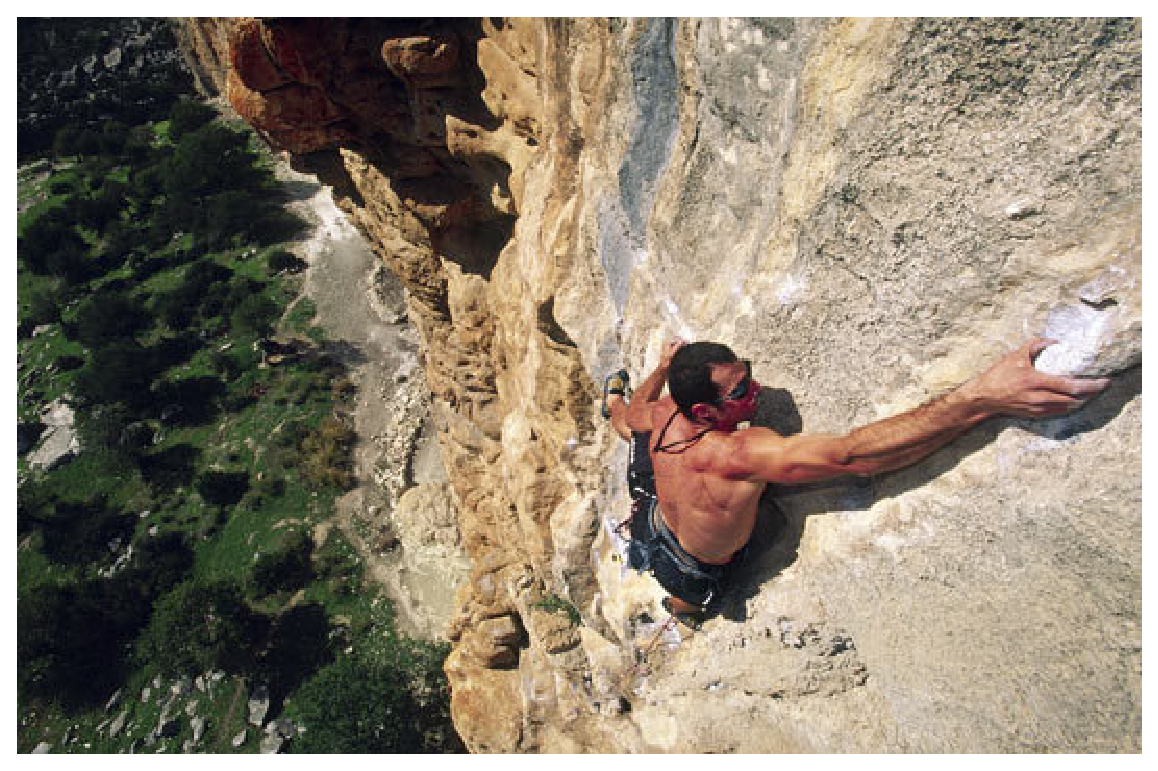
\includegraphics{lezec.eps}
			\reflectbox{\scalebox{1.18}{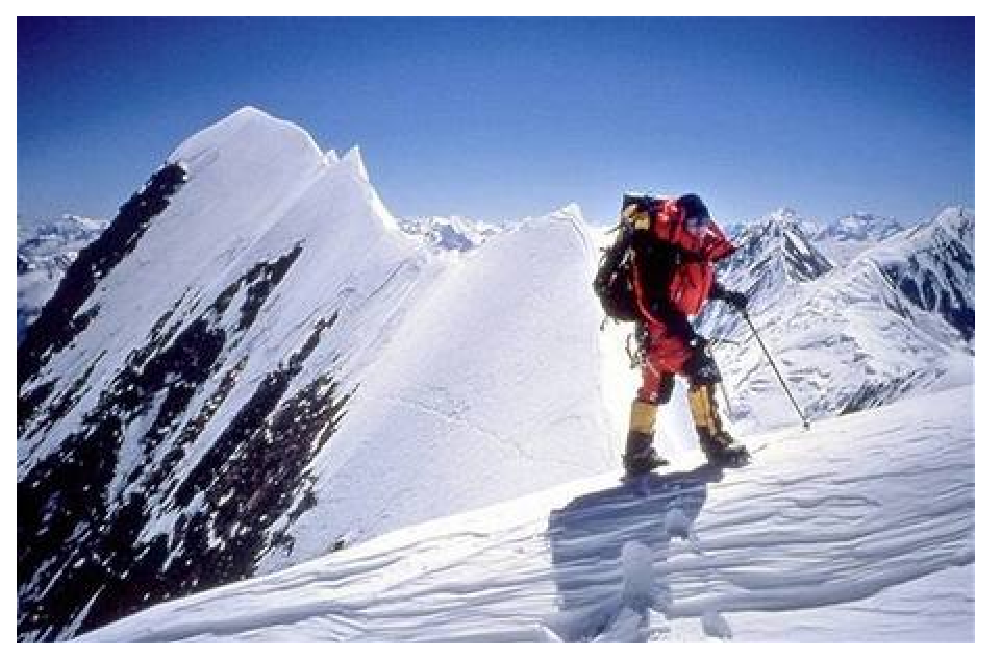
\includegraphics{horolezec.eps}}}}
			\caption{Lezec a horolezec}
		\end{center}
	\end{figure}

\end{slide}

\overlays{5}{
\begin{slide}{Štýly prelezu cesty}
	Aby sa mohli prelezi ciest porovnávať bolo nutné zaviesť štýly prelezu.
	\begin{itemize}
		\fromSlide{2}{
			\item{On sight, skrátene OS}
				\begin{itemize}
					\item{prelez štýlom RP, pričom lezec nesmie cestu poznať}
					\item{nesmie si nechať radiť od iných}
					\item{má iba jeden pokus}
				\end{itemize}
		}
		\fromSlide{3}{
			\item{Flash}
				\begin{itemize}
					\item{prelez štýlom RP bez odsadnutia, ak lezec už cestu videl liezť}
					\item{pozná ju od iných, alebo necháva si radiť}
					\item{má iba jeden pokus}
				\end{itemize}
		}
		\fromSlide{4}{
			\item{Red point, skrátene RP}
				\begin{itemize}
					\item{lezec je istený lanom z dola, a v ceste nie sú pripravené expresky}
					\item{nesmie spadnúť, alebo odpočívať na istiacich bodoch}
					\item{pri páde pokus končí neúspechom}
				\end{itemize}
		}
		\fromSlide{5}{
			\item{Pink point, skrátene PP}
				\begin{itemize}
					\item{prelez štýlom RP, ale v ceste už sú pripravené expresky}
				\end{itemize}
		}
	\end{itemize}
\end{slide} }

\overlays{2}{
\begin{slide}{Obtiažnosť ciest}
	Aby si lezec mohol pohodlne vybrať cestu, bolo nutné zaviesť klasifikačnú tabuľku.
	\begin{itemize}
		\item{UIAA}
		\item{Francúzska}
		\item{USA}
		\item{a mnoho dalších}
	\end{itemize}

	\bigskip

	\begin{table}[h]
		\begin{center}
			\begin{tabular}{|c|c|c|c|c|c|c|c|c|} \hline
				UIAA & V+  & VI- & VI  & VI+   & \ldots & XI-/XI & XI    & XI+    \\  \hline
				Fr.  & 5a  &  5b & 5c  & 6a    & \ldots & 8c+    &  9a   & 9a+     \\  \hline
				USA  & 5.7 & 5.8 & 5.9 & 5.10a & \ldots & 5.14c  & 5.14d & 5.15a    \\  \hline
			\end{tabular}
		\end{center}
	\end{table}
	\medskip
	\fromSlide{2}{
		\begin{itemize}
			\item{Čím väščie číslo, tým náročnejšia cesta.}
		\end{itemize}
	}
\end{slide} }

\begin{slide}{Trénink}
	\begin{itemize}
		\item{najlepší tréning je lezenie}
		\item{cez leto na skale, v zime na umelej stene}
	\end{itemize}

	\begin{figure}[h]
		\begin{center}
			\setlength{\unitlength}{4pt}
			\begin{picture}(40, 23)(0, 0)
				%y ova os
				\put(0, 0){\vector(0, 1){23}}
				%x ova os
				\put(0, 0){\vector(1, 0){30}}
				%ciary grafu
				%y = x
				\put(0, 0){\line(1, 1){5}}
				% y = k, rovnobezna s x
				\put(5, 5){\line(1, 0){3}}

				\put(8, 5){\line(1, 1){3}}
				\put(11, 8){\line(1, 0){3}}

				\put(14, 8){\line(1, 1){3}}
				\put(17, 11){\line(1, 0){2}}

				\put(19, 11){\line(1, 1){2.5}}
				\put(21.5, 13.5){\line(1, 0){1}}
				
				%posledna kkriva ciara
				\put(22.5, 13.5){\vector(3, 2){8}}

				%vykonnost
				\put(-7, 22){\makebox(0,0)[c]{výkonnosť}}
				%cas
				\put(28, -2){\makebox(0,0)[c]{čas}}
			\end{picture}
		\end{center}
		\caption{ideálna krivka výkonnosti}
	\end{figure}
\end{slide}

\begin{slide}{Použité zdroje}
	\begin{itemize}
		\item{Wikipedie \\ \url{http://cs.wikipedia.org/wiki/Horolezectv%C3%AD}}
		\item{G. Hattingh: Horolezectví}
	\end{itemize}
\end{slide}

\end{document}